% Block 8: Projekte nach Erfahrungsstufe
\begin{frame}{Überblick Projekte}
\begin{itemize}\setlength{\itemsep}{3mm}
  \item Fünf Stufen nach Erfahrung
  \item Projekte zum Mitnehmen
  \item Zeit 10 bis 40 Minuten
\end{itemize}
\end{frame}

% Kabel/Draht Projekt
\begin{frame}{Kabel/Draht Projekt}
\begin{columns}[T]
  \begin{column}{0.58\textwidth}
    \small
    \begin{itemize}\setlength{\itemsep}{3mm}
      \item Stufe 1: Anfänge
      \item Einfacher einstieg
      \item Lernziel: Kabel trennen, abisolieren und wieder verlöten
    \end{itemize}
    \normalsize
  \end{column}
  \begin{column}{0.42\textwidth}
    \centering
    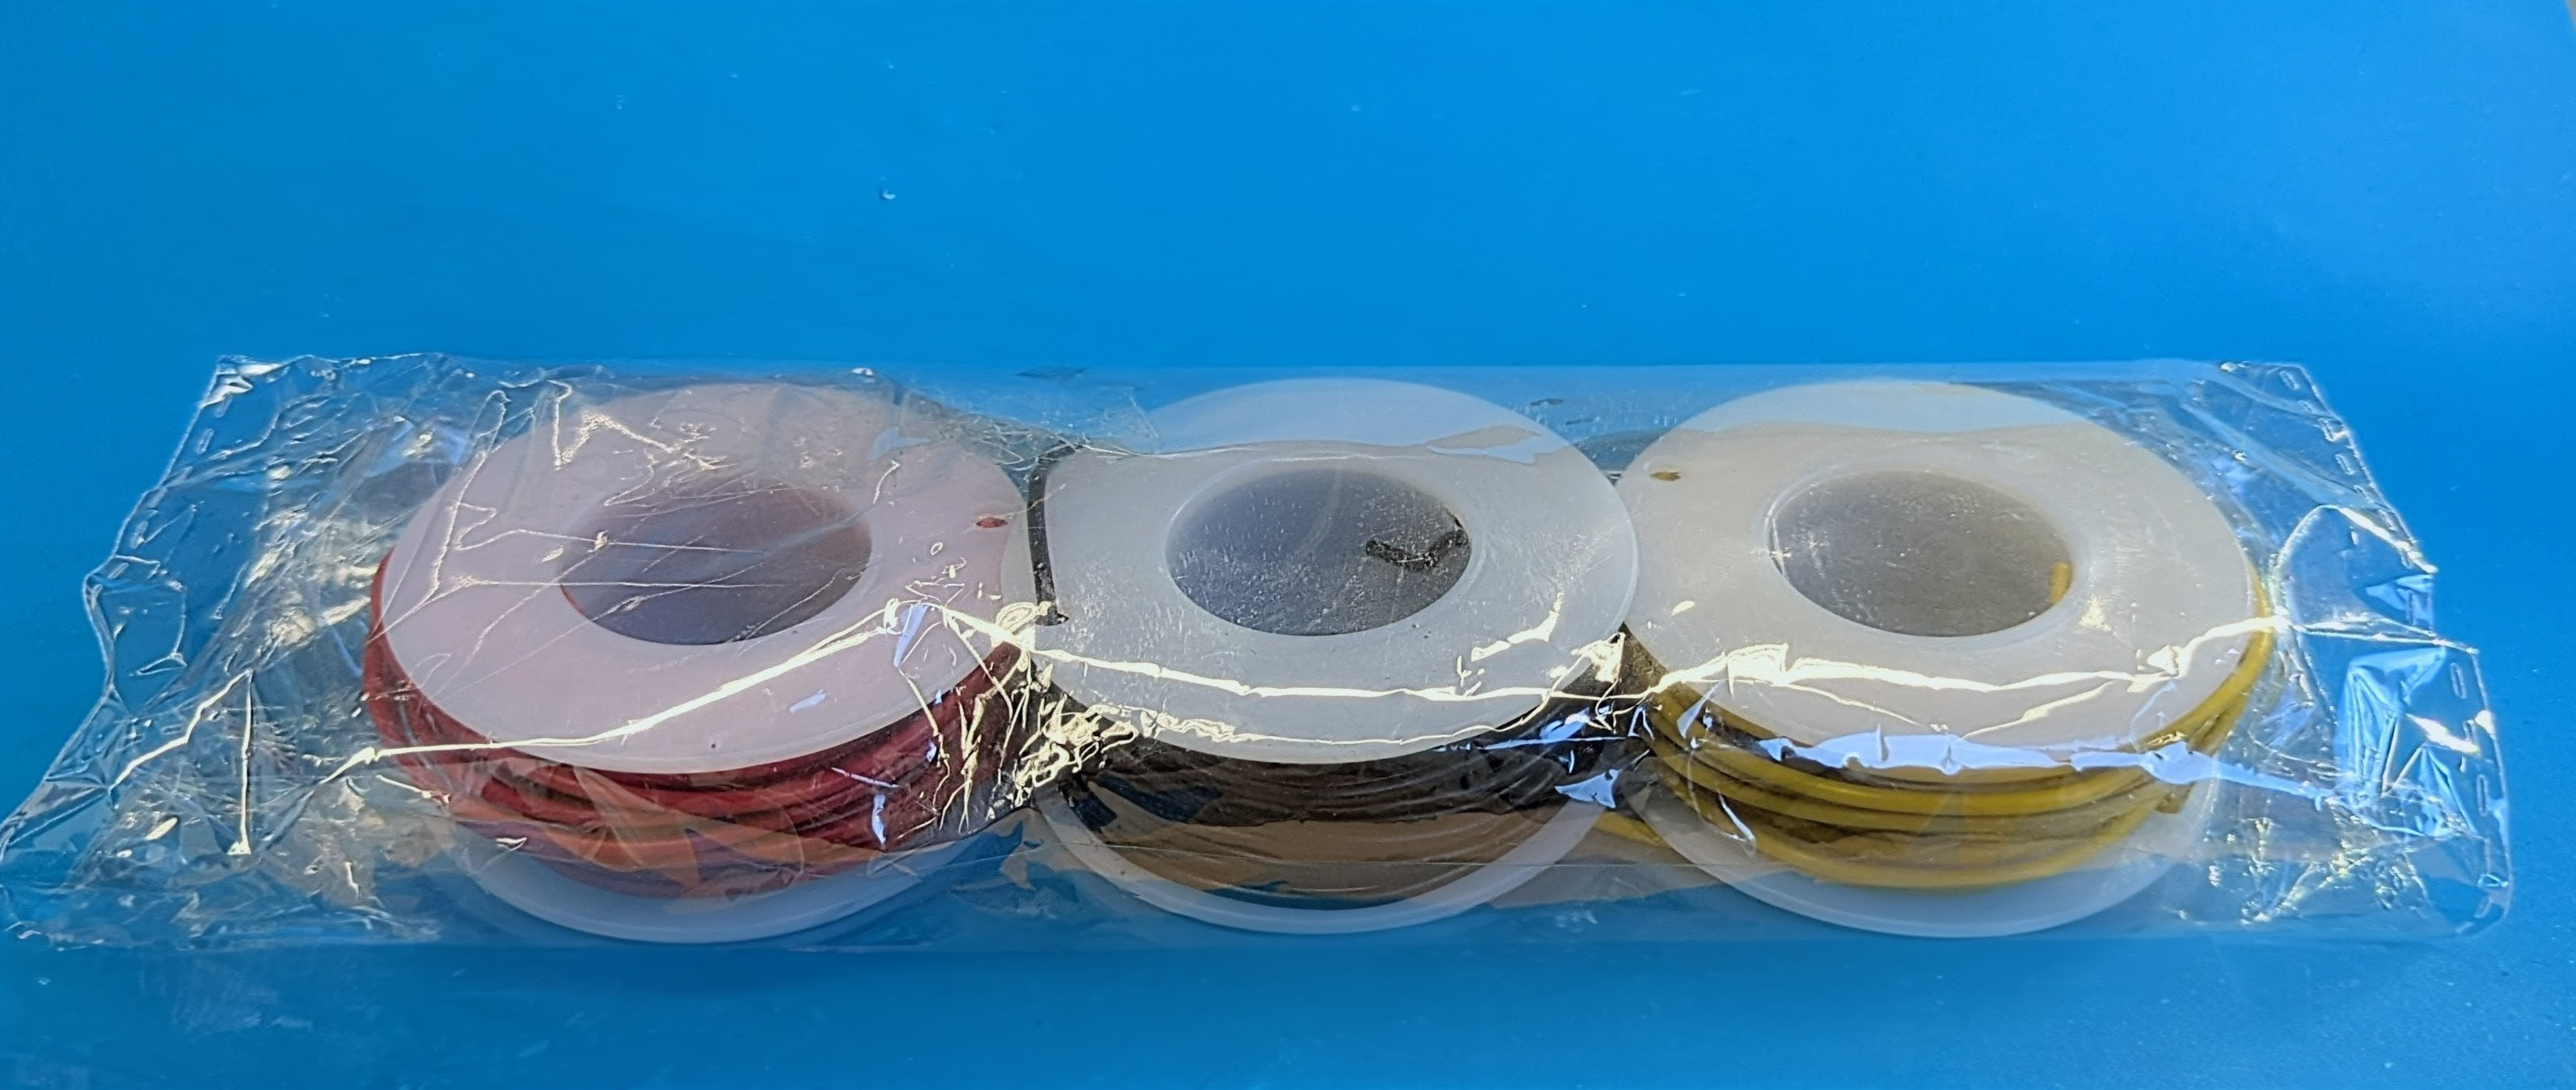
\includegraphics[width=\linewidth,keepaspectratio]{2.0.0.0_content/assets/bilder/projekt_kabel.jpg}
  \end{column}
\end{columns}
\end{frame}

\begin{frame}{Kabel fertig}
\begin{columns}[T]
  \begin{column}{0.58\textwidth}
    \small
    \begin{itemize}\setlength{\itemsep}{3mm}
      \item Sichtprüfung und Kontrolle
      \item Prüfung der elektrischen Verbindung mit Multimeter
      \item Vergleich mit Originalkabel mit Multimeter
    \end{itemize}
    \normalsize
  \end{column}
  \begin{column}{0.42\textwidth}
    \centering
    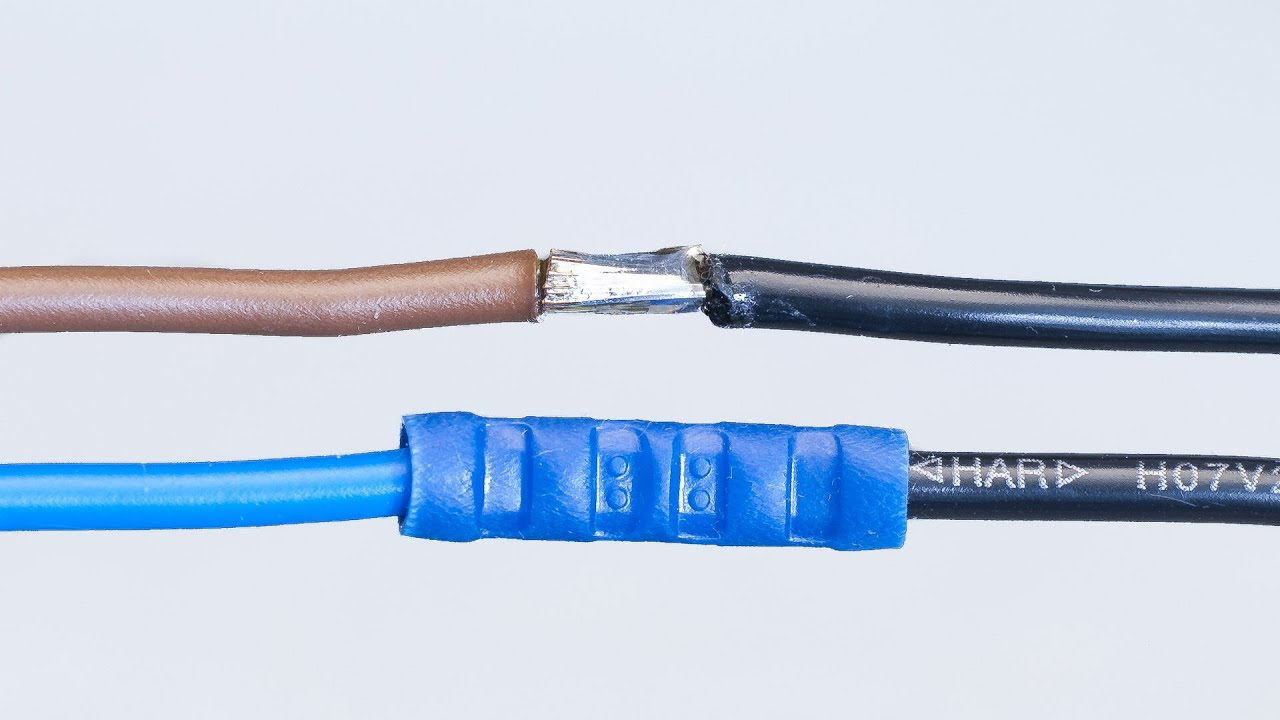
\includegraphics[width=\linewidth,keepaspectratio]{2.0.0.0_content/assets/bilder/projekt_kabel_fertig.jpg}
  \end{column}
\end{columns}
\end{frame}

% GB Projekt
\begin{frame}{GB "Nicht Tetris" Projekt}
\begin{columns}[T]
  \begin{column}{0.58\textwidth}
    \small
    \begin{itemize}\setlength{\itemsep}{3mm}
      \item Mehrteiliger Bausatz mit LED-Matrix und Tasten nur THT
      \item Saubere Lötstellen auf engem Raum benötigt
      \item Lernziel: ruhige Hand und kurze Lötzeiten
    \end{itemize}
    \normalsize
  \end{column}
  \begin{column}{0.42\textwidth}
    \centering
    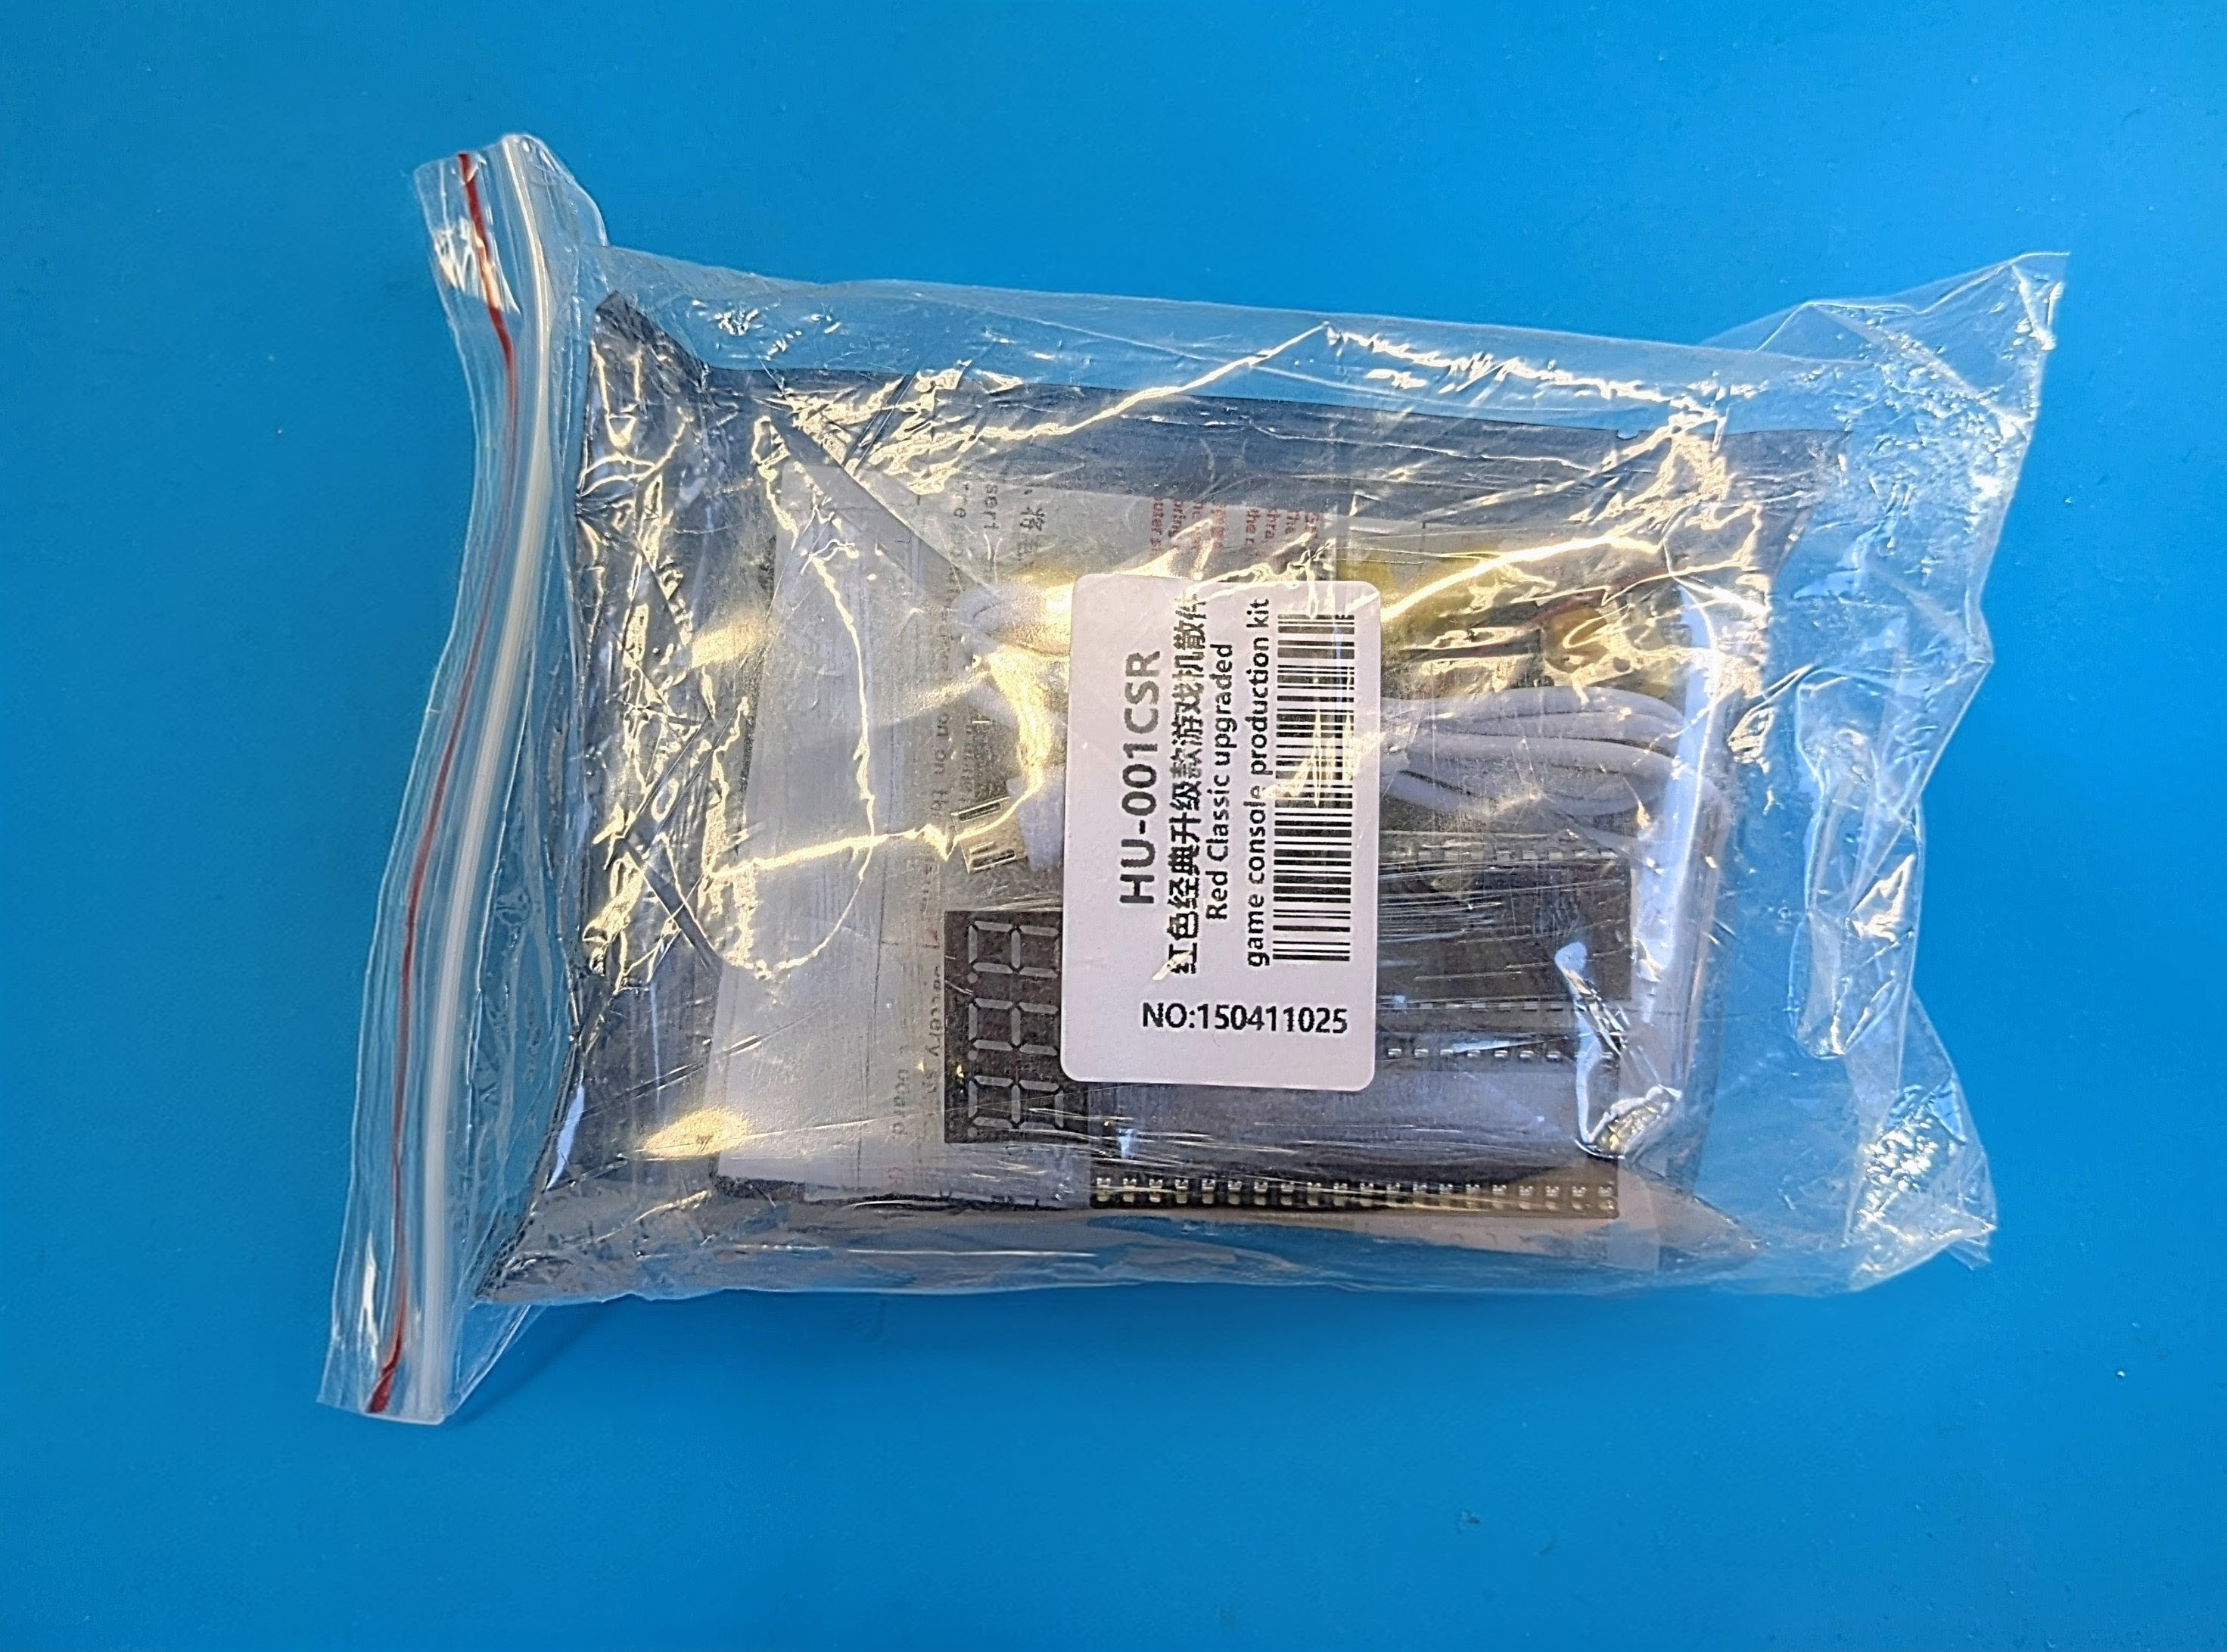
\includegraphics[width=\linewidth,keepaspectratio]{2.0.0.0_content/assets/bilder/projekt_gb_1.jpg}
  \end{column}
\end{columns}
\end{frame}

\begin{frame}{GB ’Nicht Tetris’ fertig}
\begin{columns}[T]
  \begin{column}{0.58\textwidth}
    \small
    \begin{itemize}\setlength{\itemsep}{3mm}
      \item Funktion getestet und alle Tasten reagieren
      \item Mechanisch stabil ohne Abstürze
      \item Könnt ihr narütrlich mitnehmen
    \end{itemize}
    \normalsize
  \end{column}
  \begin{column}{0.42\textwidth}
    \centering
    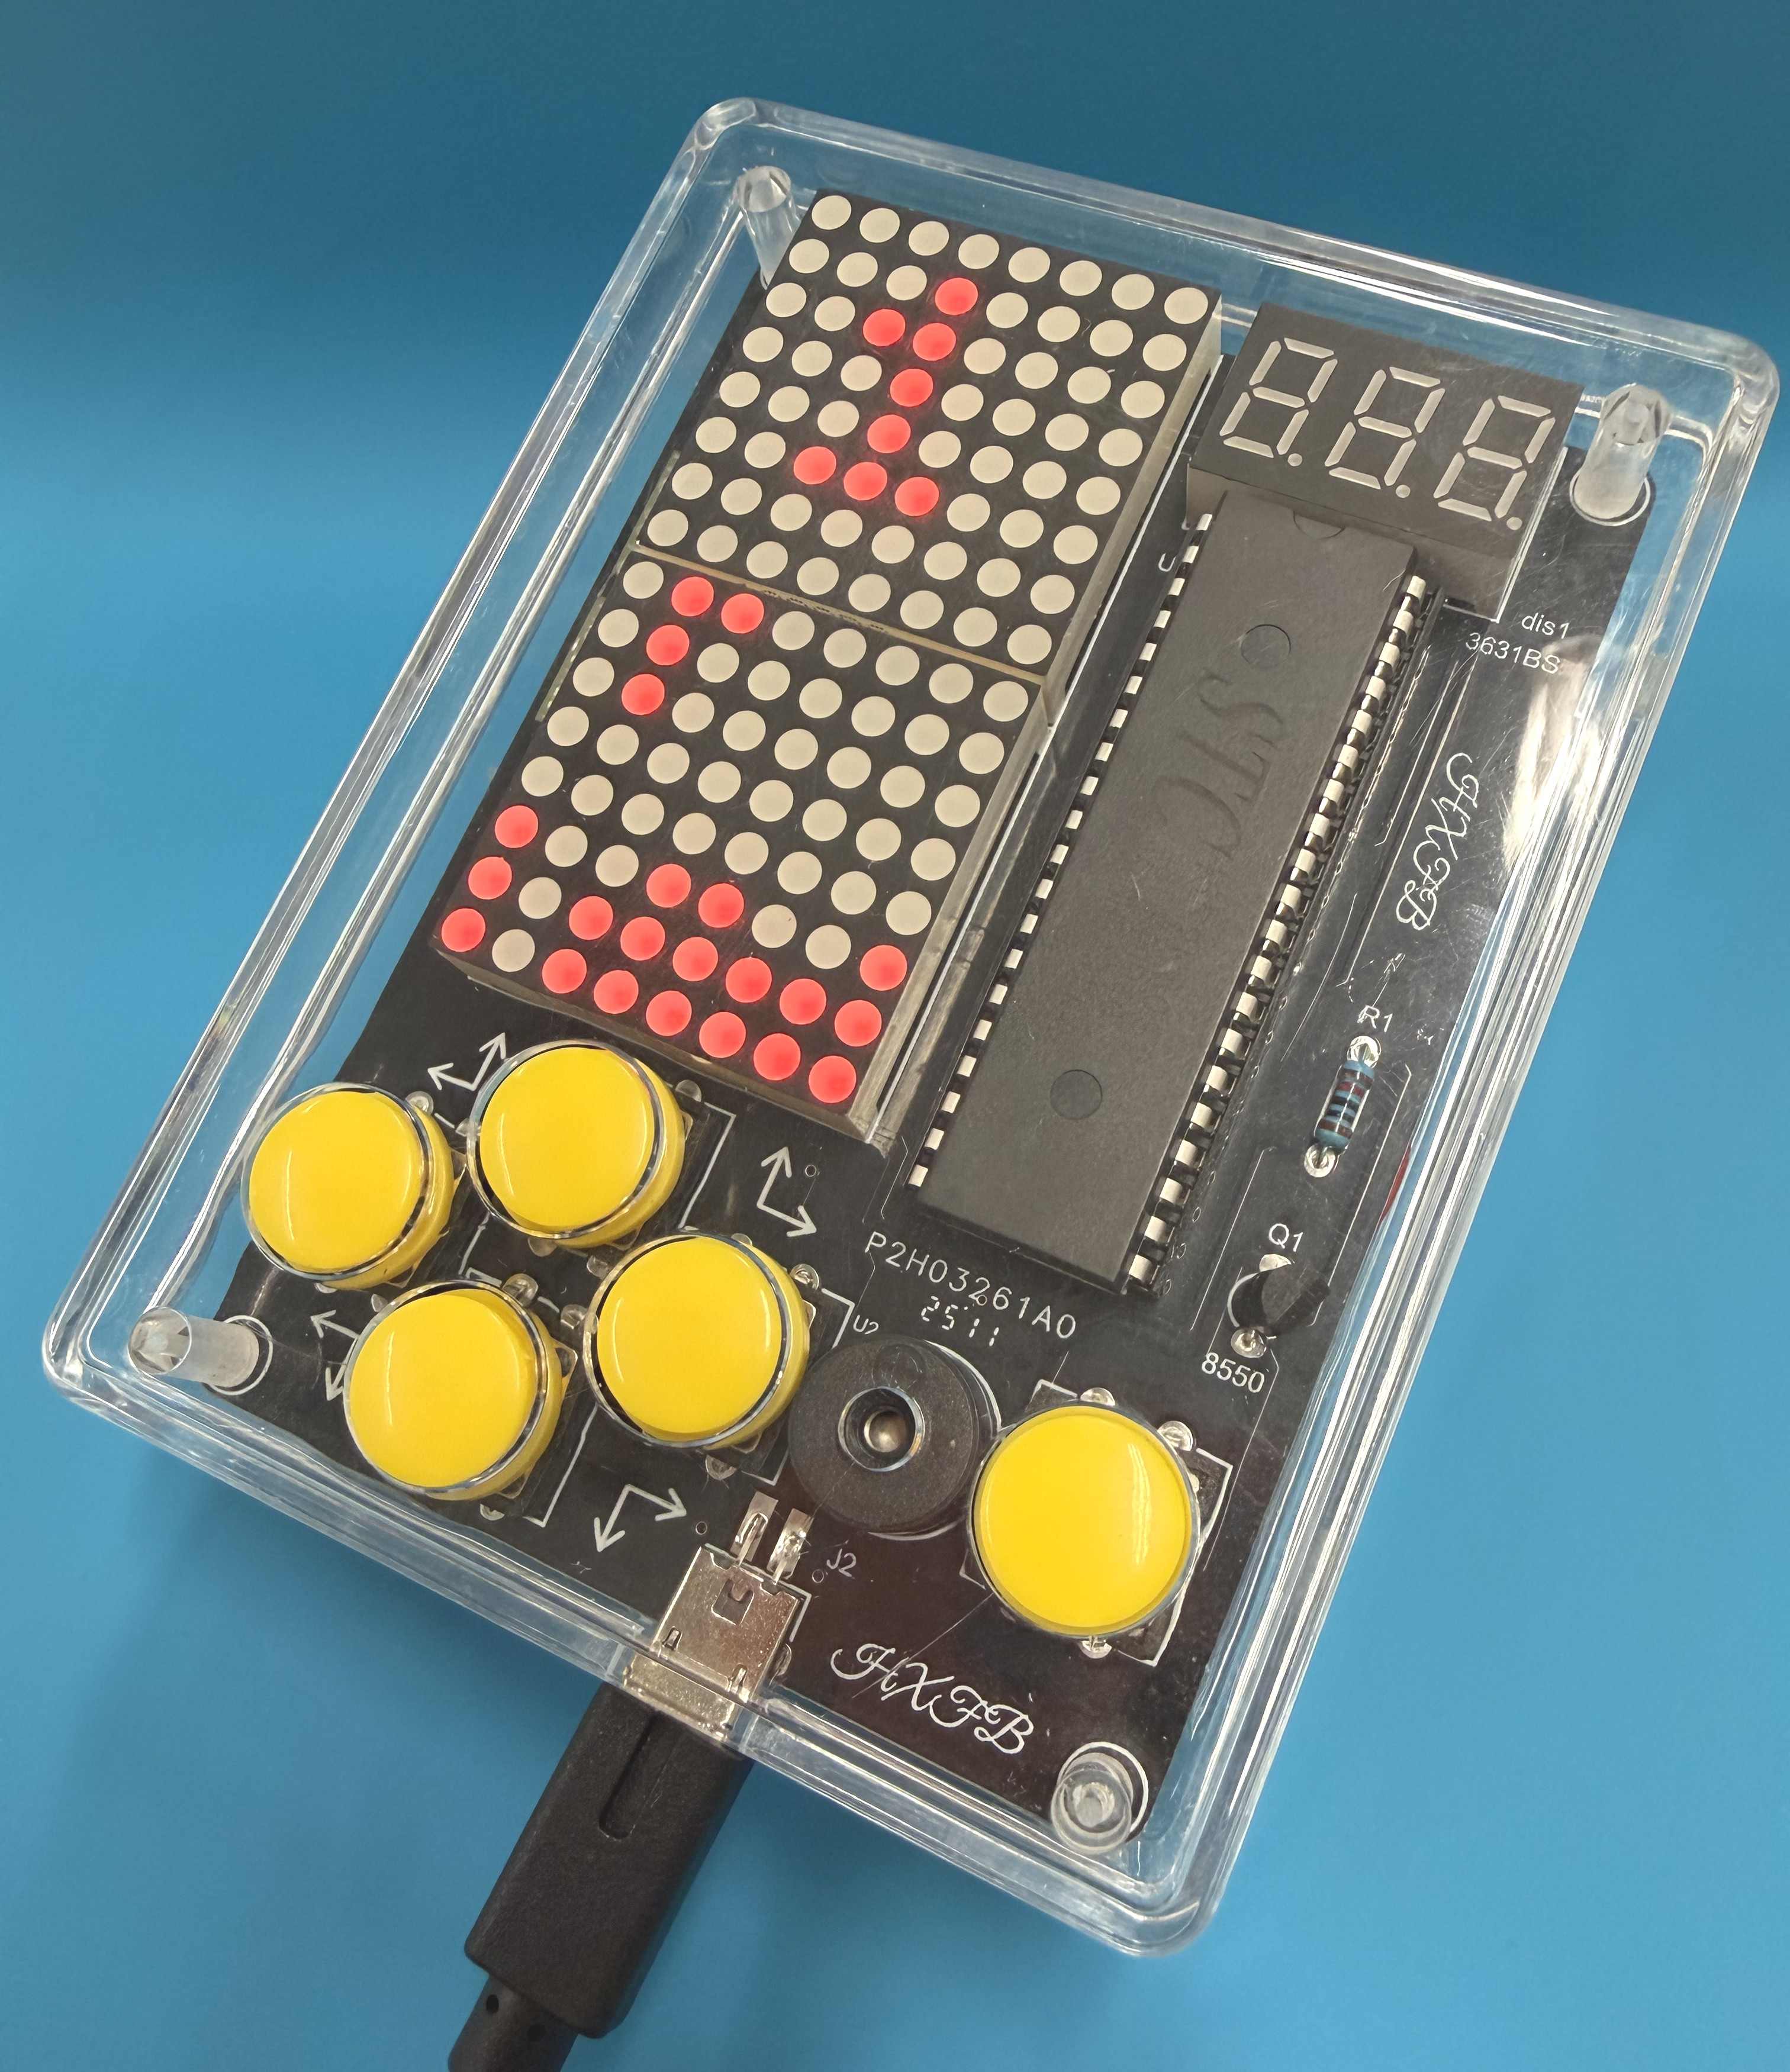
\includegraphics[width=\linewidth,keepaspectratio]{2.0.0.0_content/assets/bilder/projekt_gb_tetris_fertig_2.jpg}
  \end{column}
\end{columns}
\end{frame}


% ESP Wetter Uhr
\begin{frame}{ESP Wetter Uhr Projekt}
\begin{columns}[T]
  \begin{column}{0.58\textwidth}
    \small
    \begin{itemize}\setlength{\itemsep}{3mm}
      \item ESP Mikrocontroller mit Display
      \item Anzeige von Zeit und Wetter(mit WLAN und API)
      \item Lernziel: Stiftleisten, 3 kleine SMD/SMT und Temperaturdisziplin
    \end{itemize}
    \normalsize
  \end{column}
  \begin{column}{0.42\textwidth}
    \centering
    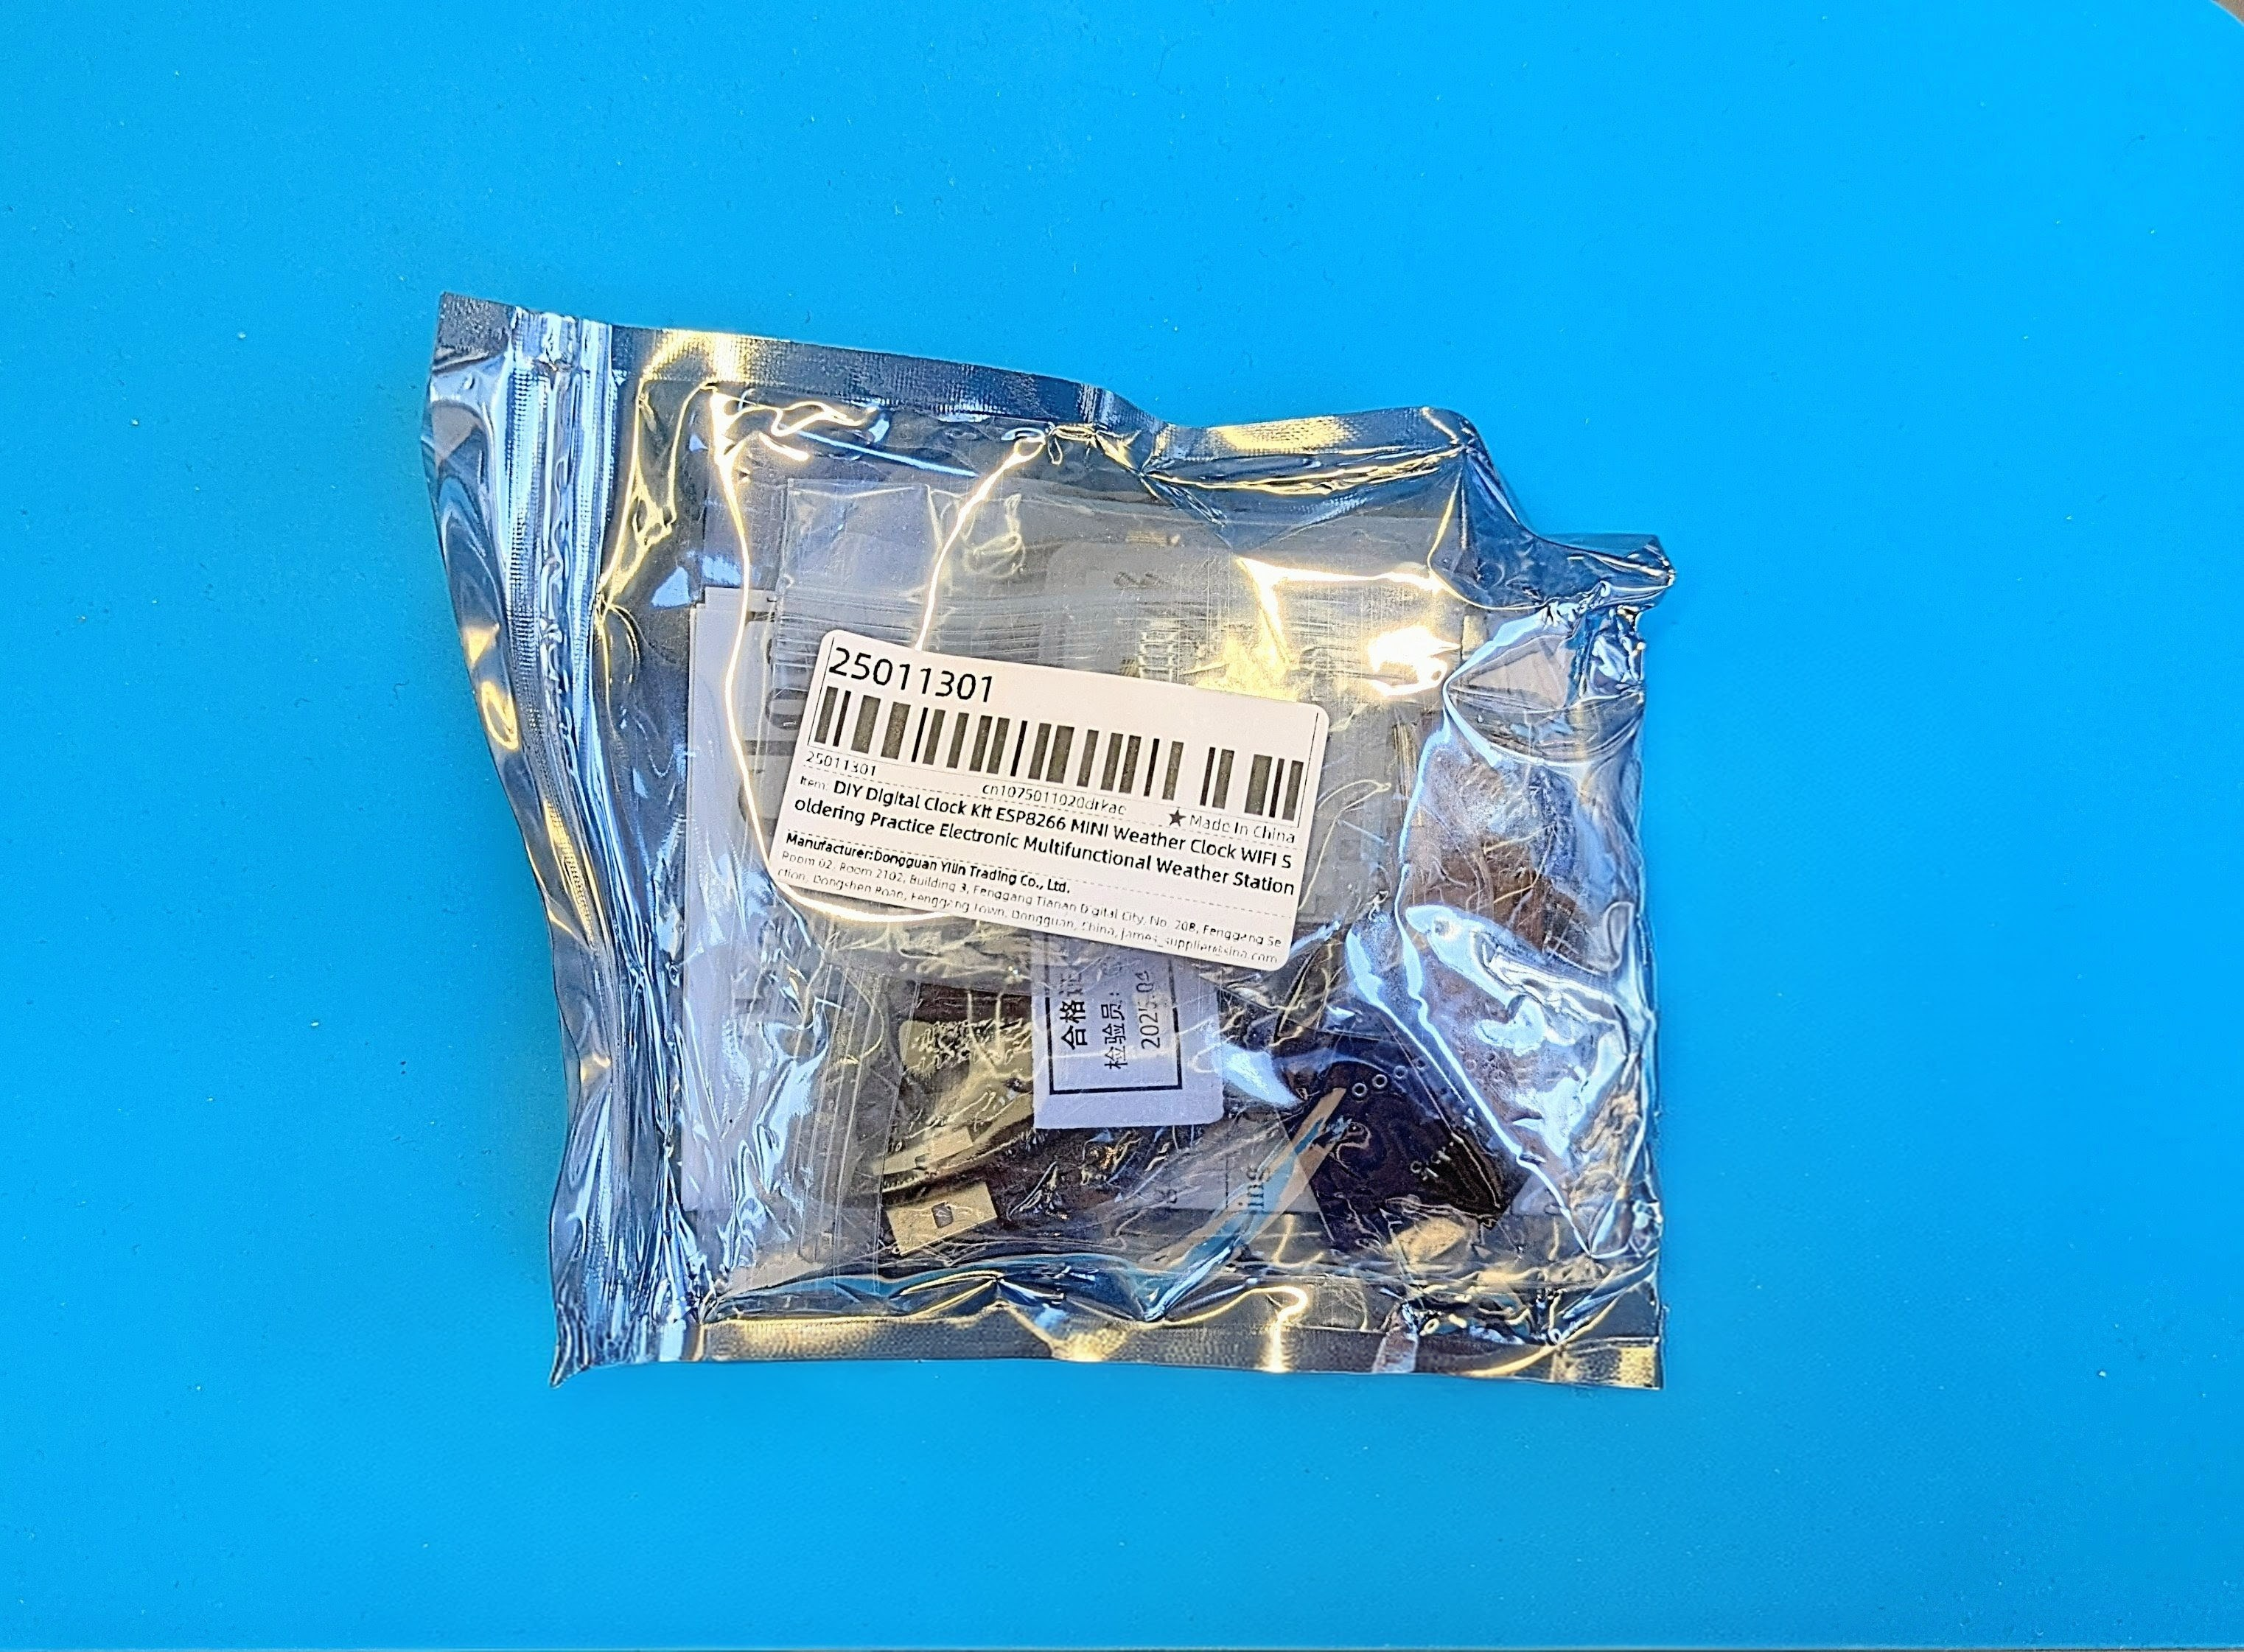
\includegraphics[width=\linewidth,keepaspectratio]{2.0.0.0_content/assets/bilder/projekt_esp_wetter_uhr_1.jpg}
  \end{column}
\end{columns}
\end{frame}

\begin{frame}{ESP Wetter Uhr fertig}
\begin{columns}[T]
  \begin{column}{0.58\textwidth}
    \small
    \begin{itemize}\setlength{\itemsep}{3mm}
      \item Anzeige getestet und lesbar
      \item Stromversorgung geprüft
      \item Bereit zum Mitnehmen
    \end{itemize}
    \normalsize
  \end{column}
  \begin{column}{0.42\textwidth}
    \centering
    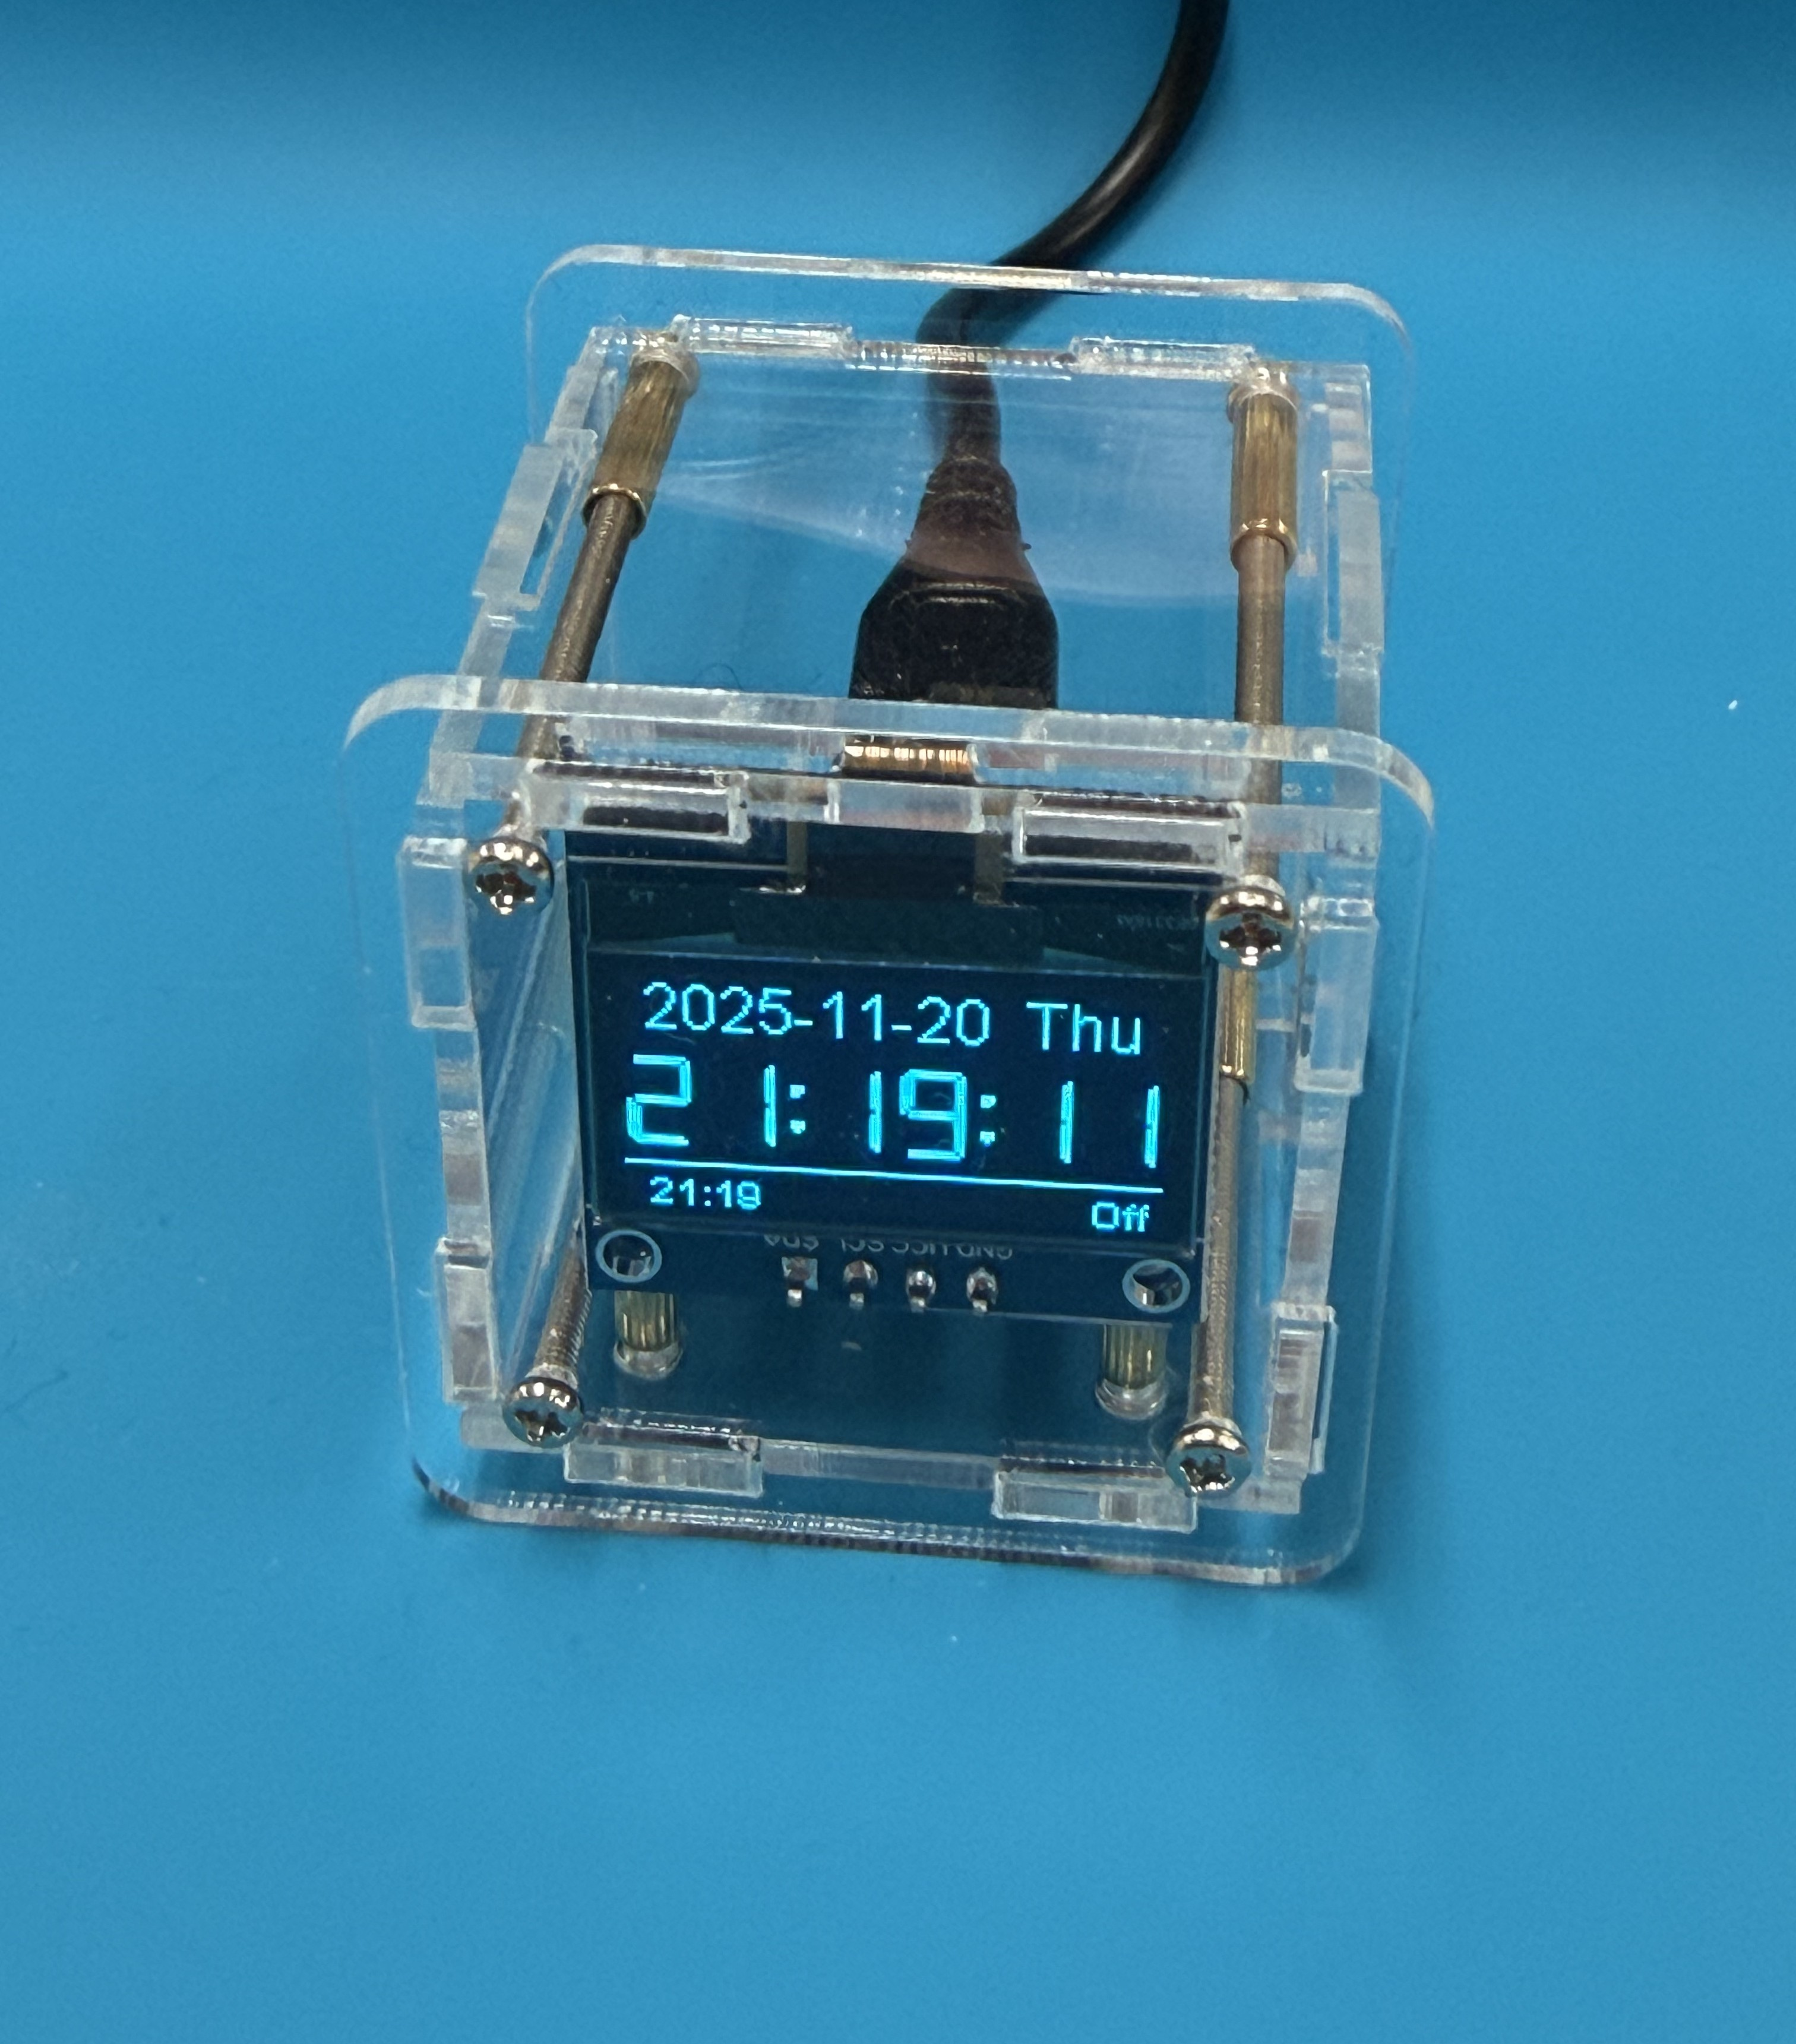
\includegraphics[width=\linewidth,keepaspectratio]{2.0.0.0_content/assets/bilder/projekt_esp_wetter_uhr_fertig.jpg}
  \end{column}
\end{columns}
\end{frame}


% Taschenrechner
\begin{frame}{Taschenrechner Projekt}
\begin{columns}[T]
  \begin{column}{0.58\textwidth}
    \small
    \begin{itemize}\setlength{\itemsep}{3mm}
      \item THT Taschenrechner Bausatz
      \item Widerstände, IC, Taster und Quarz
      \item Lernziel: Reihenfolge und saubere Wärmeführung
    \end{itemize}
    \normalsize
  \end{column}
  \begin{column}{0.42\textwidth}
    \centering
    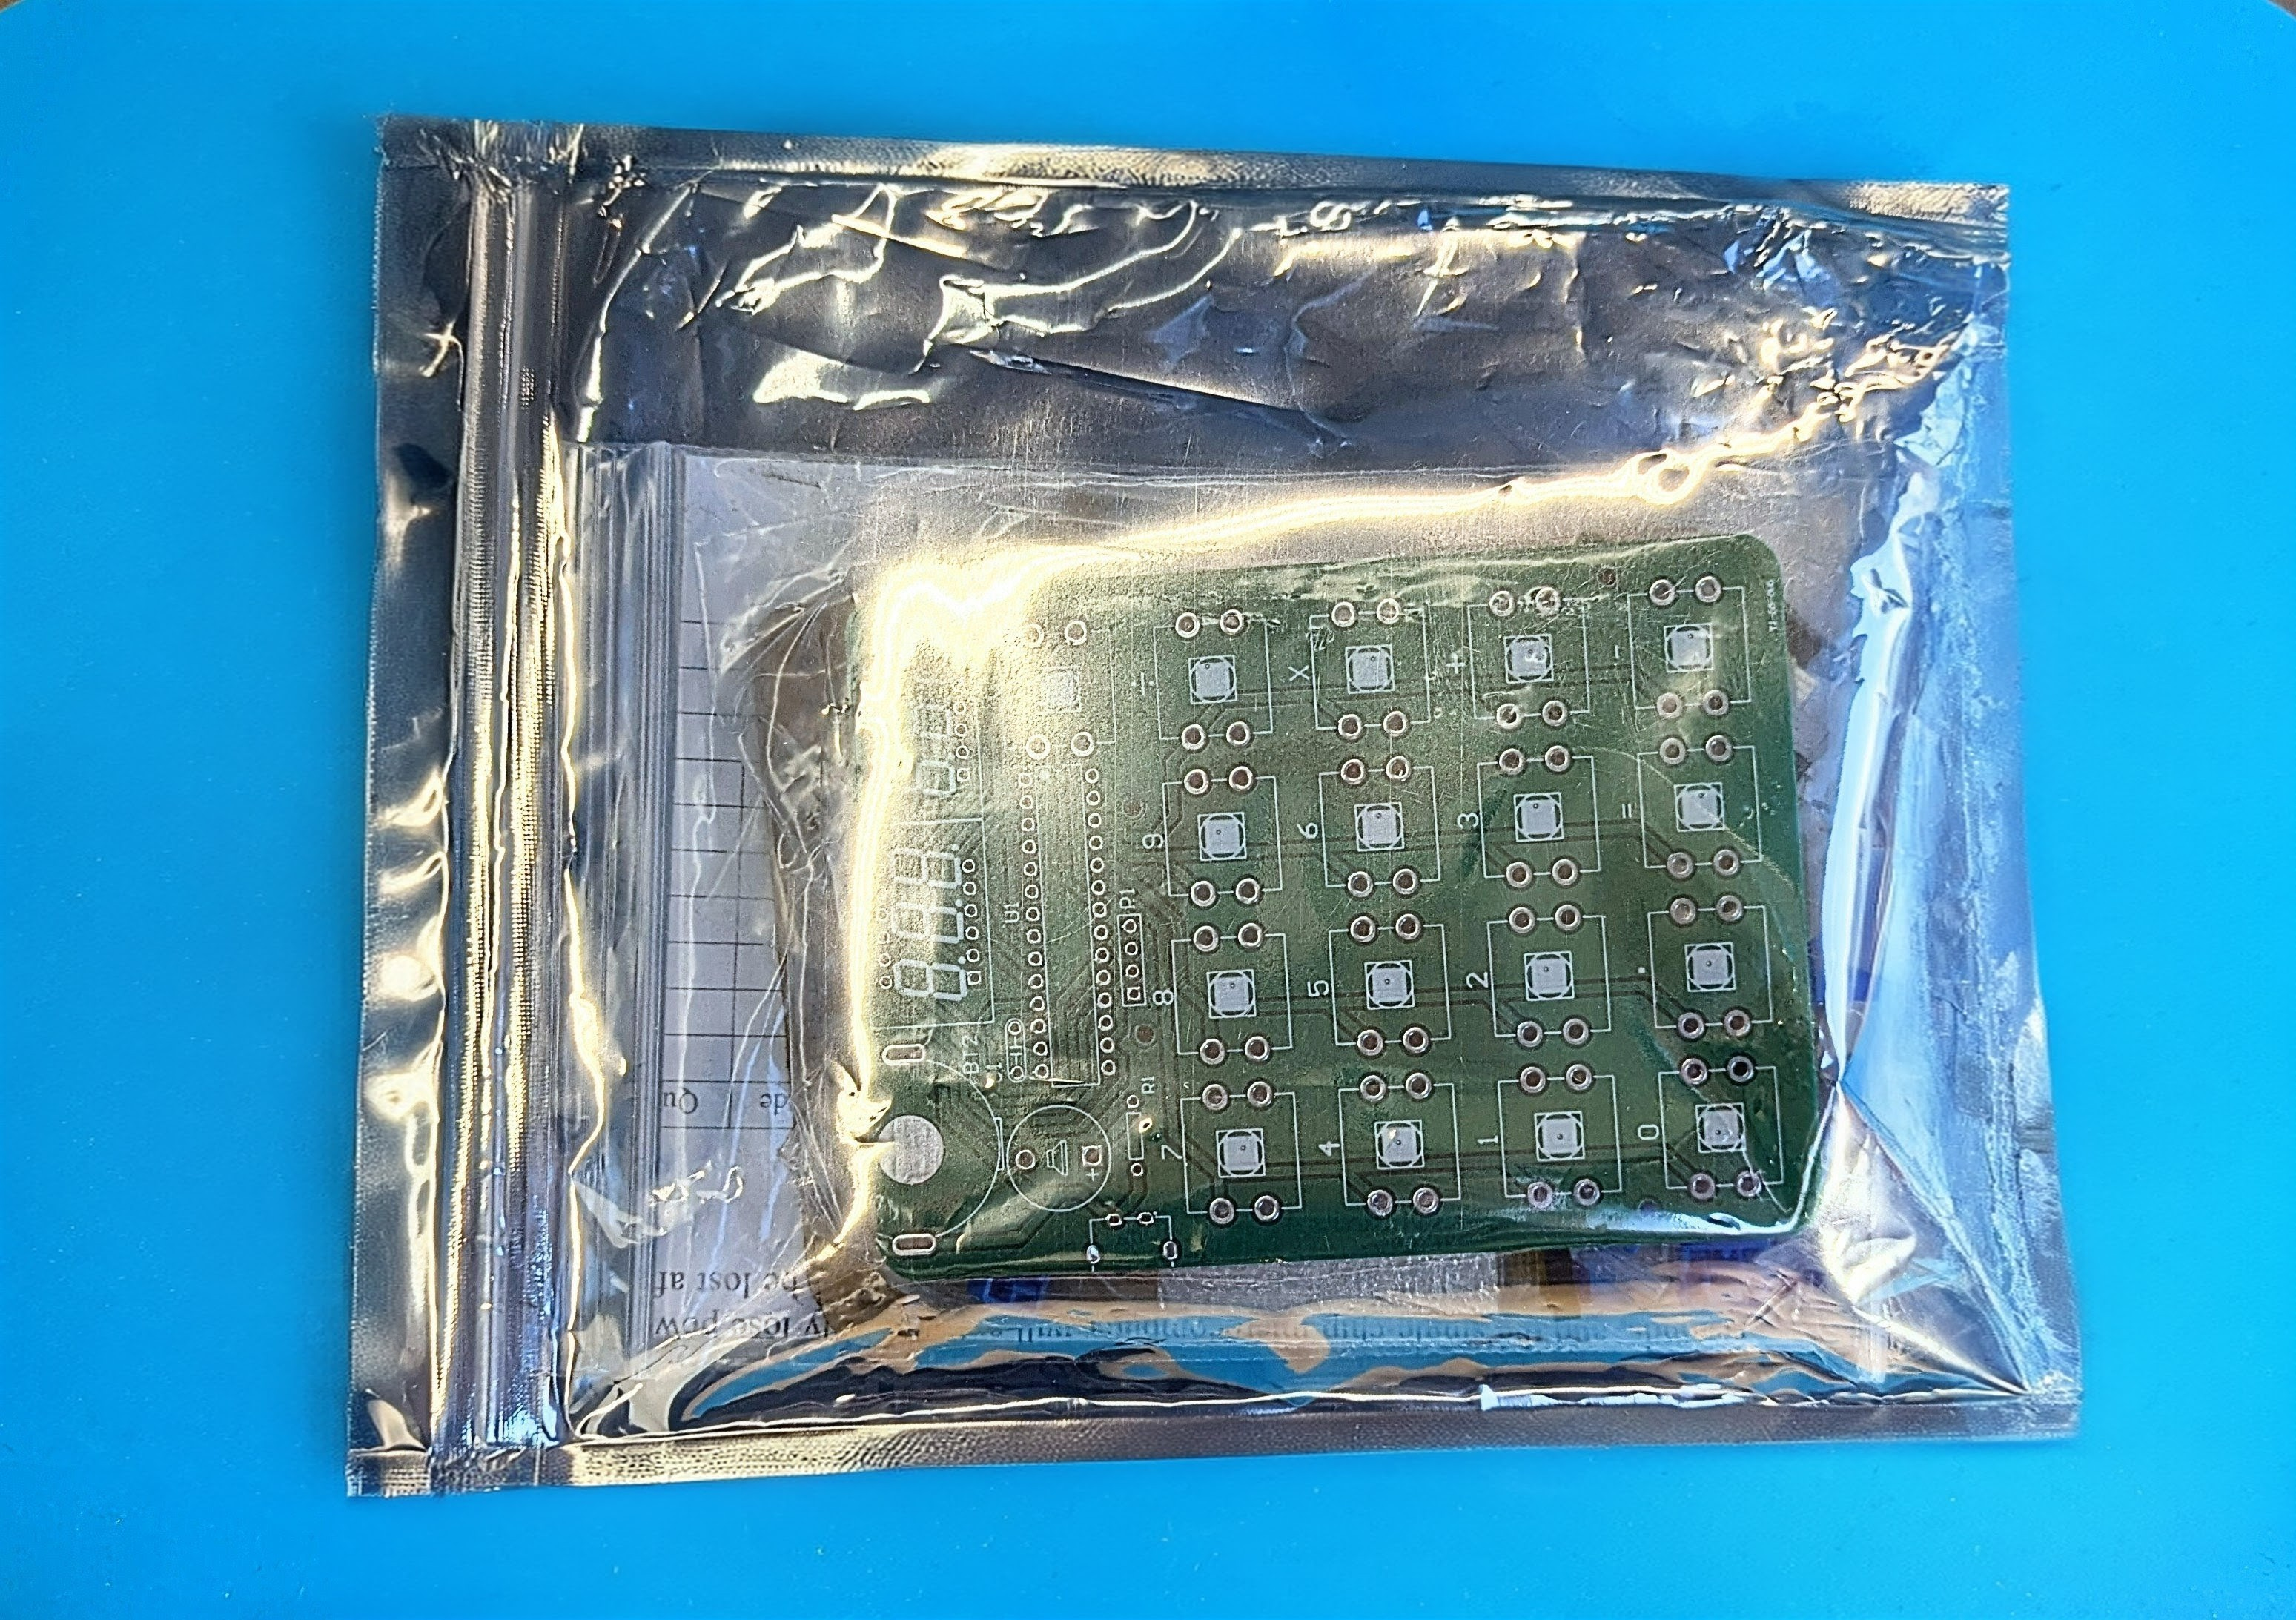
\includegraphics[width=\linewidth,keepaspectratio]{2.0.0.0_content/assets/bilder/projekt_calc.jpg}
  \end{column}
\end{columns}
\end{frame}

\begin{frame}{Taschenrechner fertig}
\begin{columns}[T]
  \begin{column}{0.58\textwidth}
    \small
    \begin{itemize}\setlength{\itemsep}{3mm}
      \item Funktion geprüft und einsatzbereit
      \item Alle Lötstellen kontrolliert
      \item Mitnahme nach kurzem Test möglich
    \end{itemize}
    \normalsize
  \end{column}
  \begin{column}{0.42\textwidth}
    \centering
    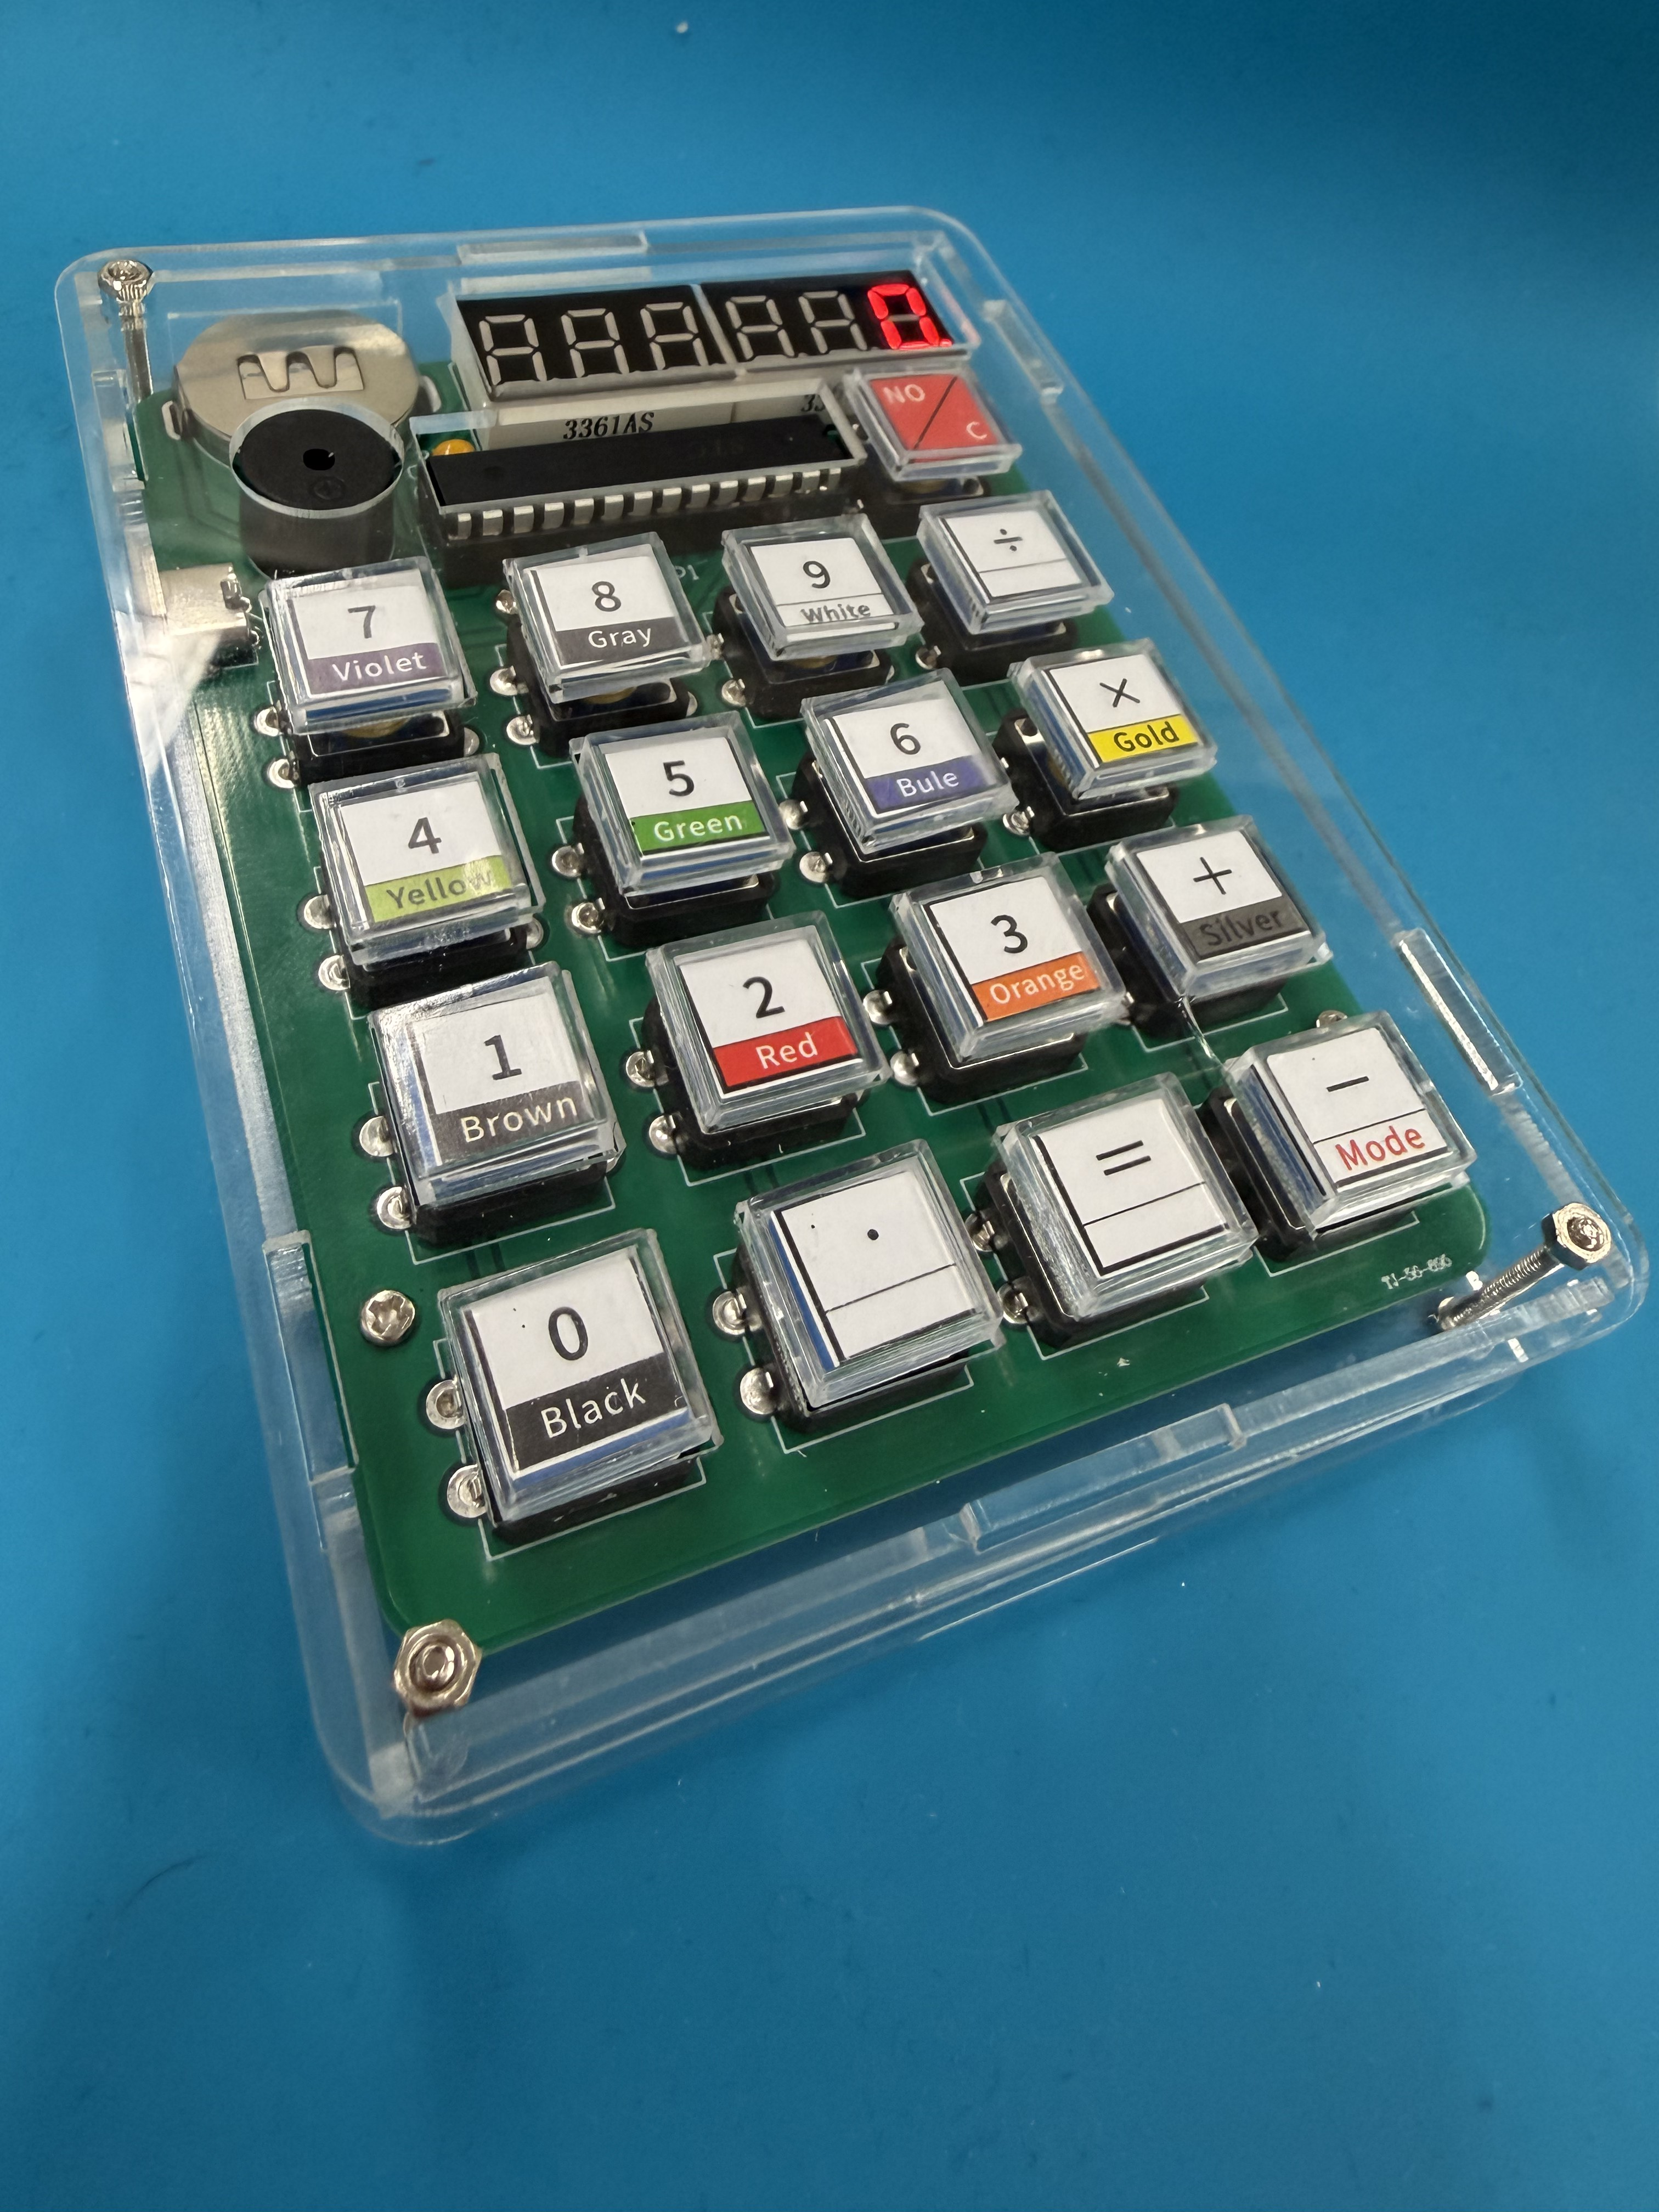
\includegraphics[width=\linewidth,keepaspectratio]{2.0.0.0_content/assets/bilder/taschenrechner_fertig_eingeschaltet.jpg}dd
  \end{column}
\end{columns}
\end{frame}

% Uhr
\begin{frame}{Uhr Projekt}
\begin{columns}[T]
  \begin{column}{0.58\textwidth}
    \small
    \begin{itemize}\setlength{\itemsep}{3mm}
      \item Digitale Uhr als Bausatz
      \item Display und mehrere THT Bauteile
      \item Lernziel: Serienlöten und Bauteilorientierung
    \end{itemize}
    \normalsize
  \end{column}
  \begin{column}{0.42\textwidth}
    \centering
    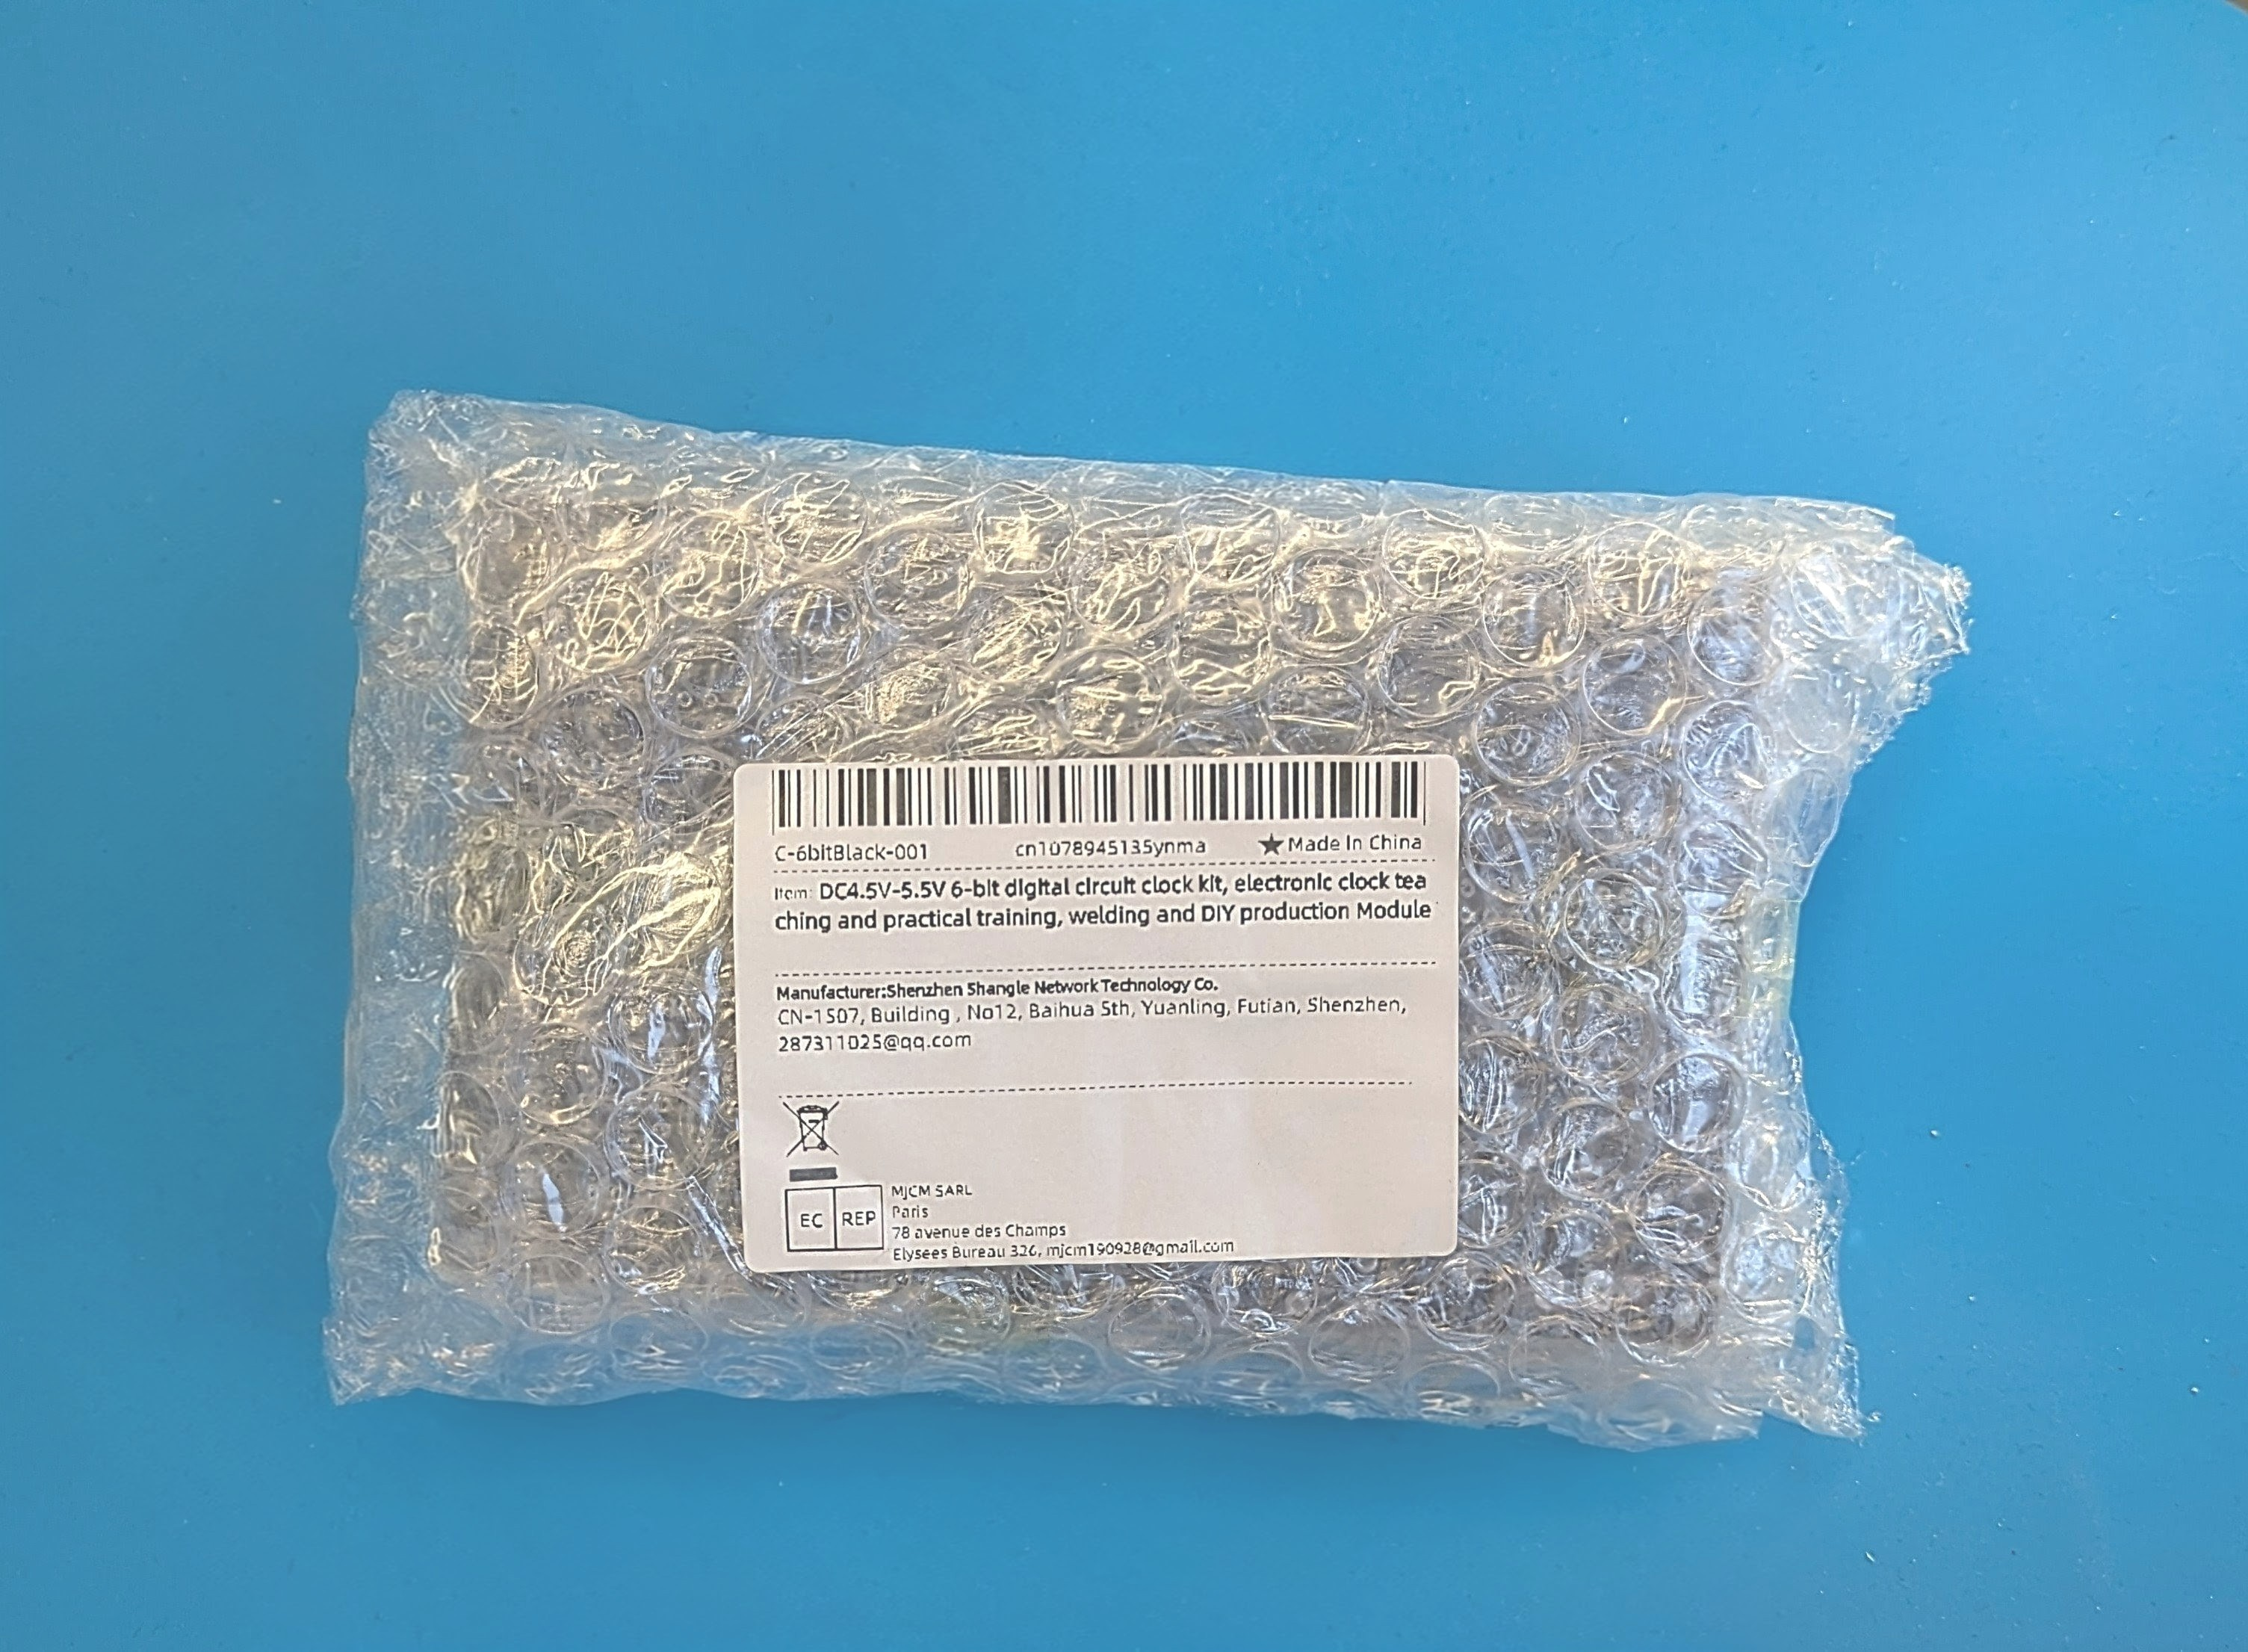
\includegraphics[width=\linewidth,keepaspectratio]{2.0.0.0_content/assets/bilder/projekt_clock.jpg}
  \end{column}
\end{columns}
\end{frame}

\begin{frame}{Uhr fertig}
\begin{columns}[T]
  \begin{column}{0.58\textwidth}
    \small
    \begin{itemize}\setlength{\itemsep}{3mm}
      \item Uhr läuft stabil
      \item Saubere Lötstellen ohne Brücken
      \item Optionales Gehäuse möglich
    \end{itemize}
    \normalsize
  \end{column}
  \begin{column}{0.42\textwidth}
    \centering
    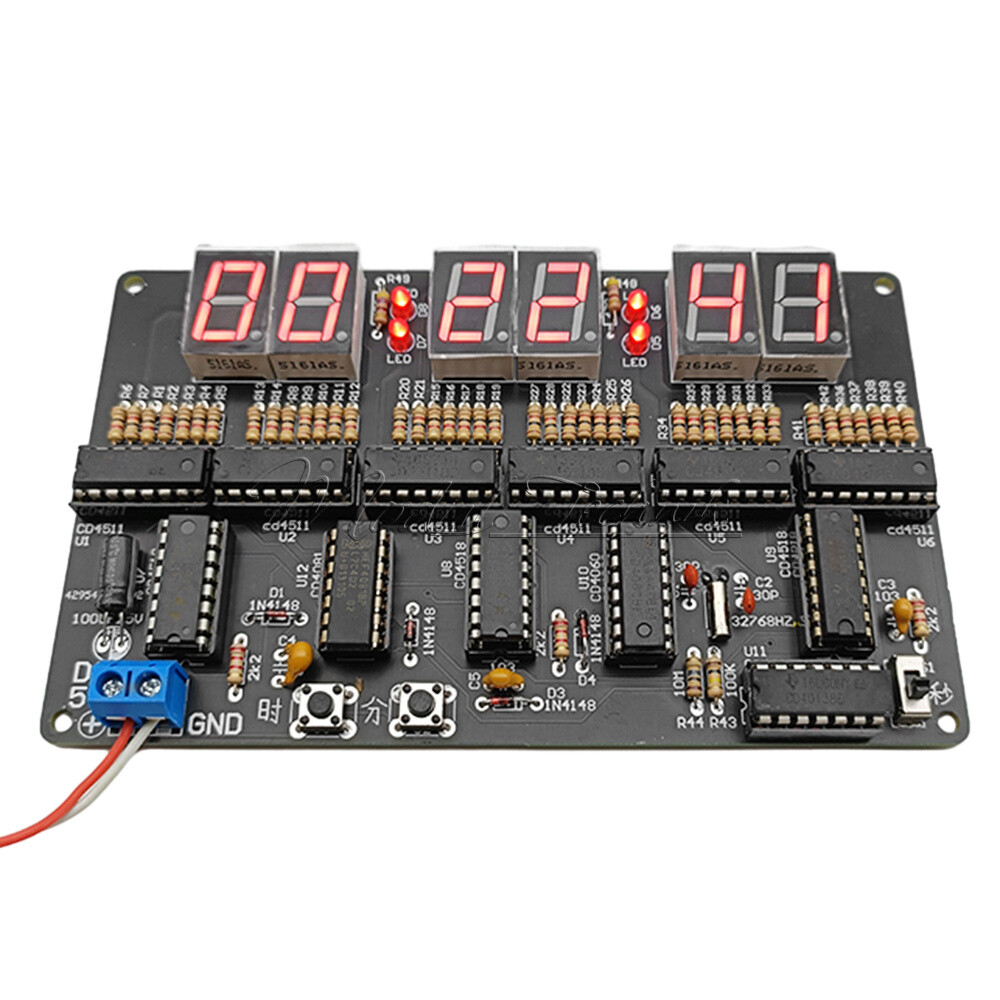
\includegraphics[width=\linewidth,keepaspectratio]{2.0.0.0_content/assets/bilder/projekt_clock_fertig.jpg}
  \end{column}
\end{columns}
\end{frame}

\begin{frame}{Projektvorstellung kurz}
\begin{itemize}\setlength{\itemsep}{3mm}
  \item \textbf{Was macht das Projekt} und was ist am Ende sichtbar oder nutzbar
  \item \textbf{Welche Teile} werden gelötet und worauf muss man achten
  \item \textbf{Woran erkennt man den Erfolg}, also zum Beispiel Licht, Anzeige oder Funktion
\end{itemize}
\end{frame}

\begin{frame}{Sicherheit bei Projekten}
\begin{itemize}\setlength{\itemsep}{3mm}
  \item Immer die \textbf{passende Temperatur} wählen
  \item \textbf{Bauteile nicht überhitzen} und lieber kurz als zu lange erhitzen
  \item Nach jedem Schritt \textbf{prüfen}, bevor weitergelötet wird
\end{itemize}
\end{frame}

\begin{frame}{Material und Rückgabe}
\begin{itemize}\setlength{\itemsep}{3mm}
  \item Teile werden je nach \textbf{Projektstufe} ausgegeben
  \item \textbf{Reste sortiert sammeln} und den Arbeitsplatz ordentlich halten
  \item Werkzeug bitte \textbf{vollständig und sauber} zurücklegen
\end{itemize}
\end{frame}

\begin{frame}{Q \& A}
\begin{itemize}\setlength{\itemsep}{3mm}
  \item Fragen zum \textbf{Pinecil} oder zu den Einstellungen
  \item Fragen zu \textbf{Projekten}, \textbf{Fehlern} oder \textbf{Bauteilen}
  \item Tipps für \textbf{eigene Projekte zu Hause}
\end{itemize}
\end{frame}

\begin{frame}{Humor und Motivation}
\begin{itemize}\setlength{\itemsep}{3mm}
  \item \textbf{Merke:} Lötzinn, nicht Blödsinn
  \item Das Ziel ist ein \textbf{sicherer und guter Einstieg}, nicht maximale Geschwindigkeit
  \item Und wenn etwas nicht klappt: \textbf{Wir helfen dir gern}
\end{itemize}
\end{frame}



